% ============================================================
%  CHAPITRE 2 : CONCEPT ET ÉTUDE PRÉALABLE

\chapter{Concepts de base et étude préalable}

\minitoc

\newpage

% ------------------------------------------------------------
\section{Introduction}
% ------------------------------------------------------------

Après avoir présenté le contexte général du projet, l'étude de l'existant, les exigences ainsi que la méthodologie de travail adoptée, ce chapitre introduit les fondements théoriques et les choix d'architecture de la solution proposée.

La plateforme repose sur plusieurs concepts clés de l'intelligence artificielle moderne, notamment les modèles de langage (LLMs), les systèmes multi-agents, le Retrieval-Augmented Generation (RAG), les embeddings, les prompts système et les agent skills, qui constituent la base du fonctionnement des agents intelligents.

Le chapitre présente également le système de mémoire persistante basé sur Hindsight, ainsi que l'architecture globale de la solution et ses principaux choix techniques, afin de préparer la phase d'implémentation.

% ------------------------------------------------------------
\section{Fondements de l'intelligence artificielle}
% ------------------------------------------------------------

La plateforme développée dans le cadre de ce projet repose sur plusieurs concepts fondamentaux de l'intelligence artificielle moderne qui constituent la base de son fonctionnement.

Les sections suivantes présentent les principaux fondements mobilisés, notamment les modèles de langage de grande taille, les agents intelligents et les systèmes multi-agents, les représentations vectorielles sémantiques, les prompts système et les agent skills.

\subsection{Les modèles de langage de grande taille (LLMs)}

Les modèles de langage de grande taille (LLMs) occupent une place essentielle dans les systèmes d'intelligence artificielle modernes. Leur compréhension est indispensable pour comprendre leur intégration et leur rôle au sein de la plateforme.

\subsubsection{Définition des LLMs}

Un grand modèle de langage \cite{cloudflare_llm} (Large Language Model, LLM) est un modèle d'intelligence artificielle entraîné sur de très vastes corpus de données textuelles afin d'apprendre les structures statistiques et sémantiques du langage naturel. Il est capable de comprendre, générer et manipuler du texte avec un haut niveau de cohérence, en produisant des sorties adaptées au contexte d'entrée.

\subsubsection{Utilisation dans le projet}

Dans la plateforme, les LLMs sont utilisés comme moteur principal des fonctionnalités intelligentes. Ils interviennent notamment dans :

\begin{itemize}
    \item la génération de contenus pédagogiques,
    \item l'analyse des requêtes des utilisateurs,
    \item la production de réponses contextualisées,
    \item la génération d'activités personnalisées.
\end{itemize}

Ces modèles ne sont pas exploités de manière isolée. Ils sont intégrés dans un pipeline applicatif enrichi par un contexte métier (cours, progression de l'apprenant, objectifs pédagogiques), et leurs sorties peuvent être structurées (ex. JSON) afin d'être exploitées par les différents modules du système.

\subsubsection{Étude du choix du LLM}

Le choix du modèle de langage repose sur plusieurs critères : qualité des réponses, capacité à gérer de longs contextes, coût d'utilisation, facilité d'intégration et compatibilité avec les besoins du projet.

Une comparaison de plusieurs modèles a été réalisée afin d'identifier la solution la plus adaptée aux contraintes de la plateforme (tableau~\ref{tab:comparaison_llm}).

\begin{table}[H]
\centering
\caption{Étude comparative des LLMs}
\label{tab:comparaison_llm}
\renewcommand{\arraystretch}{1.25}
\resizebox{\textwidth}{!}{%
\begin{tabular}{|p{4.0cm}|p{2.8cm}|p{2.7cm}|p{2.8cm}|p{5.6cm}|}
\hline
\textbf{Modèle} & \textbf{Fournisseur} & \textbf{Nombre de paramètres} & \textbf{Fenêtre de contexte} & \textbf{Coût du LLM} \\
\hline
openai/gpt-oss-120b:free \cite{openai_gpt_oss} & OpenRouter / OpenAI OSS & 117 milliards & 131K tokens \cite{openrouter_gpt_oss_free} & 0 \$ / 1M tokens en entrée ; 0 \$ / 1M tokens en sortie \cite{openrouter_gpt_oss_free} \\
\hline
gemma-4-4b & Serveur interne de la société & 4 milliards & Non communiqué publiquement & 0 \$ / 1M tokens en entrée ; 0 \$ / 1M tokens en sortie \\
\hline
GPT-5.4 mini \cite{openai_gpt54_mini_intro} & OpenAI & Non communiqué & 400K tokens \cite{openai_gpt54_mini_intro} & 0,75 \$ / 1M tokens en entrée ; 4,50 \$ / 1M tokens en sortie \cite{openai_api_pricing} \\
\hline
Claude Haiku 4.5 \cite{anthropic_haiku} & Anthropic & Non communiqué & 200K tokens \cite{anthropic_haiku_system_card} & 1 \$ / 1M tokens en entrée ; 5 \$ / 1M tokens en sortie \cite{anthropic_pricing} \\
\hline
Gemini 3.1 Flash-Lite \cite{cloudflare_gemini_31_flash_lite} & Google / Gemini & Non communiqué & 1M tokens \cite{cloudflare_gemini_31_flash_lite} & 0,25 \$ / 1M tokens en entrée ; 1,50 \$ / 1M tokens en sortie \cite{google_gemini_pricing} \\
\hline
Llama 3.1 8B Instant \cite{groq_llama_31_8b_model} & Groq & 8 milliards & 131072 tokens \cite{groq_llama_31_8b_model} & 0,05 \$ / 1M tokens en entrée ; 0,08 \$ / 1M tokens en sortie \cite{groq_pricing} \\
\hline
Mistral Small 4 \cite{mistral_small_4_model_card} & Mistral AI & Non communiqué & 256K tokens \cite{mistral_small_4_model_card} & 0,10 \$ / 1M tokens en entrée ; 0,30 \$ / 1M tokens en sortie \cite{mistral_pricing} \\
\hline
\end{tabular}%
}
\end{table}

\subsubsection{Choix retenu}

Le modèle retenu est \textit{openai/gpt-oss-120b:free}, accessible via OpenRouter. Il est utilisé comme modèle principal pour la génération de contenus pédagogiques, l'assistance aux utilisateurs et la production de réponses contextualisées.

Ce choix s'explique par :

\begin{itemize}
    \item sa grande fenêtre de contexte (131K tokens),
    \item son coût nul en version gratuite,
    \item sa capacité à produire des réponses structurées.
\end{itemize}

Un modèle interne de l'entreprise a également été considéré, mais son usage reste limité au réseau interne, ce qui réduit sa flexibilité lors du développement et des tests. Il est donc conservé comme solution complémentaire.

\subsection{Les agents intelligents et les systèmes multi-agents}

Les agents intelligents sont une brique essentielle des systèmes IA modernes, permettant de structurer des comportements autonomes basés sur les LLMs.

Cette section présente leur rôle ainsi que celui des systèmes multi-agents dans l'architecture de la plateforme.

\subsubsection{Définition des agents intelligents}

Un agent intelligent \cite{google_ai_agents} peut être défini comme un composant logiciel
fondé sur l'intelligence artificielle, conçu pour analyser un contexte, prendre des décisions
et exécuter des actions afin d'atteindre un objectif donné. Contrairement à un programme
déterministe classique, il peut s'appuyer sur des mécanismes de raisonnement, de planification,
de mémoire et d'adaptation pour produire un comportement plus autonome.

Dans les systèmes récents basés sur les modèles de langage de grande taille, le LLM joue
souvent le rôle de moteur de raisonnement. L'agent, quant à lui, est défini par son rôle, ses
outils, sa mémoire, ses consignes et son intégration dans un processus applicatif.

\subsubsection{Définition des systèmes multi-agents}

Un système multi-agents \cite{google_multi_agent_system} correspond à une architecture dans
laquelle plusieurs agents spécialisés interviennent au sein d'un même environnement logiciel.
Chaque agent prend en charge une responsabilité précise, échange des informations avec les
autres composants du système et contribue à la réalisation d'un objectif global.

Cette approche permet de remplacer une logique centralisée par une organisation distribuée,
dans laquelle chaque agent possède un rôle clair. Elle favorise ainsi la séparation des
responsabilités, la modularité et l'évolution progressive du système.

\subsubsection{Utilisation dans le projet}

Dans le cadre de ce projet, une approche multi-agents a été adoptée afin de structurer les différentes fonctionnalités intelligentes de la plateforme. Elle permet de répartir les responsabilités entre plusieurs agents spécialisés, chacun intervenant sur un aspect précis du système.

Cette organisation permet d'éviter une logique centralisée unique et favorise la modularité ainsi que l'évolution indépendante des fonctionnalités IA.

Les principaux agents intégrés dans la plateforme sont : l'agent de création de cours, l'agent de coaching pédagogique, l'agent de mémoire apprenant, l'agent de recommandation et l'agent de défis personnalisés.

Ainsi, cette architecture multi-agents assure une meilleure spécialisation des traitements tout en maintenant une cohérence globale du système

\subsection{Le Retrieval-Augmented Generation (RAG)}

Le Retrieval-Augmented Generation (RAG) est un mécanisme important utilisé dans la plateforme pour améliorer les réponses des modèles de langage.

Cette section présente son principe général et son intégration dans le projet.

\subsubsection{Définition du RAG}

Le Retrieval-Augmented Generation (RAG) \cite{aws_rag} est une approche qui consiste à enrichir la génération d'un LLM par des informations récupérées depuis une source de connaissances externe. Au lieu de produire une réponse uniquement à partir des connaissances apprises pendant son entraînement, le modèle reçoit d'abord des éléments pertinents issus d'une base documentaire, d'une base de données ou d'une mémoire spécialisée. Ces informations sont ensuite ajoutées au contexte de la requête afin de guider la génération de la réponse.

\subsubsection{Workflow général}

Le fonctionnement général d'un système RAG suit plusieurs étapes. Les données utiles sont d'abord préparées, découpées en fragments et transformées en représentations exploitables pour la recherche, généralement à l'aide d'embeddings. Lorsqu'un utilisateur formule une requête, le système recherche les fragments les plus pertinents dans la base de connaissances, puis les injecte dans le prompt transmis au LLM. Le modèle génère alors une réponse en s'appuyant à la fois sur la question de l'utilisateur et sur le contexte récupéré. La figure~\ref{fig:rag_workflow} illustre les différentes étapes de ce processus.

\begin{figure}[H]
    \centering
    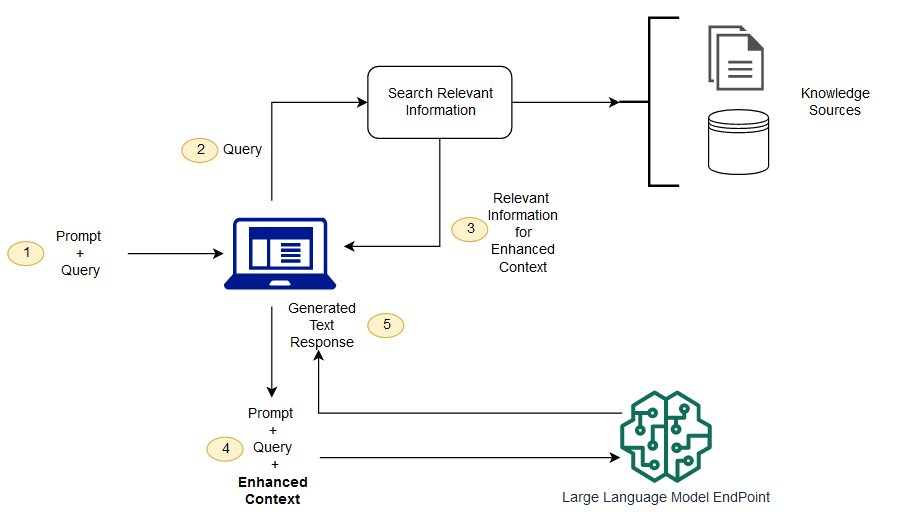
\includegraphics[width=0.85\textwidth]{figures/rag_workflow.jpg}
    \caption{Workflow général d'un système RAG \cite{aws_rag}}
    \label{fig:rag_workflow}
\end{figure}

\subsubsection{Agentic RAG}

L'\textit{agentic RAG} \cite{ibm_agentic_rag} désigne une évolution du RAG dans laquelle la récupération d'information n'est pas seulement déclenchée de manière automatique, mais pilotée par un ou plusieurs agents capables de décider quelles sources consulter, quels outils utiliser et comment intégrer les informations récupérées dans leur raisonnement. Cette approche rend le RAG plus flexible qu'un pipeline classique, car l'agent peut adapter la récupération au contexte de la requête.

\subsubsection{Utilisation dans le projet}

Dans la plateforme, l'Agentic RAG est utilisé pour les fonctionnalités nécessitant une forte contextualisation, notamment le coaching pédagogique, les recommandations, les défis personnalisés et l'exploitation de la mémoire des cours et des apprenants. Il permet aux agents de récupérer les informations pertinentes en fonction du contexte utilisateur et de l'objectif pédagogique.

Cette approche est plus adaptée qu'un RAG classique, car chaque agent (coaching, recommandation, défis) exploite un contexte différent. L'Agentic RAG permet ainsi d'adapter dynamiquement la récupération d'informations à chaque responsabilité, afin de produire des réponses plus cohérentes et personnalisées.

\subsection{Modèles d’Embeddings}

Les embeddings jouent un rôle central dans la recherche sémantique et le RAG.

Cette section en présente le principe et l’utilisation dans le projet.

\subsubsection{Définition des embeddings}

Les incorporations \cite{ibm_embedding}, ou embeddings, désignent des représentations vectorielles denses de données textuelles dans un espace mathématique de haute dimension. Elles permettent de représenter des objets, tels que du texte, des images ou de l'audio, sous forme de points dans un espace vectoriel continu dont la position porte une signification sémantique. Dans le cas du texte, la proximité géométrique entre deux vecteurs reflète ainsi une similarité de sens entre les éléments représentés.

\subsubsection{Embeddings et recherche sémantique}

Dans les systèmes basés sur les Transformers, les embeddings représentent des passages entiers et non seulement des mots isolés. Ils permettent ainsi la recherche sémantique, où le système compare le sens des requêtes et des contenus plutôt que des mots-clés exacts. Dans un système RAG, cette représentation sert à retrouver les fragments de connaissances les plus proches de la requête de l'utilisateur.

\subsubsection{Étude du choix du modèle d'embeddings}

Le choix du modèle d'embeddings influence la qualité de la recherche sémantique dans le système RAG. Une comparaison des principaux modèles est présentée dans le tableau~\ref{tab:comparaison_embeddings} selon plusieurs critères techniques et économiques.

\begin{table}[H]
\centering
\caption{Comparaison des modèles d'embeddings utilisables pour le système RAG}
\label{tab:comparaison_embeddings}
\renewcommand{\arraystretch}{1.25}
\resizebox{\textwidth}{!}{%
\begin{tabular}{|p{4.3cm}|p{3.2cm}|p{2.5cm}|p{7.0cm}|}
\hline
\textbf{Modèle} & \textbf{Fournisseur} & \textbf{Dimension} & \textbf{Coût et déploiement} \\
\hline
BAAI/bge-small-en-v1.5 \cite{baai_bge_small} & Local / SentenceTransformers & 384 & Gratuit à l'usage, exécution locale, modèle léger d'environ 130 Mo \\
\hline
text-embedding-3-small \cite{openai_embedding_models} & OpenAI & 1536 & Service cloud payant : 0,02 \$ / 1M tokens \cite{openai_embedding_pricing} \\
\hline
mistral-embed \cite{mistral_embed_models} & Mistral AI / LiteLLM & 1024 & Service cloud payant : 0,10 \$ / 1M tokens en entrée \cite{mistral_embed_model_card} \\
\hline
embed-english-v3.0 \cite{cohere_embed_models} & Cohere & 1024 & Service cloud avec clé API ; prix public par token non précisé pour ce modèle dans la page officielle \cite{cohere_pricing} \\
\hline
gemini-embedding-001 \cite{google_vertex_embeddings} & Google / Vertex AI & 3072 par défaut, dimension configurable & Service cloud : gratuit en free tier, puis 0,15 \$ / 1M tokens en entrée \cite{google_gemini_pricing} \\
\hline
\end{tabular}%
}
\end{table}

\subsubsection{Choix retenu}

À partir de cette comparaison, le modèle \textit{BAAI/bge-small-en-v1.5} a été retenu pour
la génération des embeddings dans le système RAG du projet. Ce choix s'explique par son
exécution locale, son coût nul à l'usage et sa légèreté, puisqu'il produit des vecteurs de
384 dimensions.

Ce modèle offre un compromis adapté entre qualité de recherche sémantique, consommation
mémoire et simplicité d'intégration. Les tests réalisés ont montré qu'il répond aux besoins de
récupération d'informations de la plateforme. Il est également cohérent avec le système de
mémoire utilisé dans le projet, qui supporte les embeddings locaux basés sur ce modèle
\cite{hindsight_models}.

\subsection{Les prompts système des agents IA}

Cette section présente les prompts système des agents IA ainsi que leur utilisation dans la plateforme.

\subsubsection{Définition}

Un prompt système \cite{kern_system_prompt} correspond à un ensemble de consignes placées
en amont de l'interaction avec le LLM. Il permet d'orienter le modèle avant même la demande
de l'utilisateur, en précisant le rôle attendu, les règles de comportement, le style de réponse,
les contraintes fonctionnelles et les limites à ne pas dépasser.

\subsubsection{Rôle dans les agents IA}

Dans une application basée sur des agents IA, le prompt système permet de spécialiser un
modèle généraliste afin qu'il adopte un comportement cohérent avec un contexte métier précis.
Chaque agent reçoit ainsi des consignes qui définissent son périmètre d'action, les informations
à prendre en compte et la forme attendue de sa réponse.

\subsubsection{Utilisation dans le projet}

Dans ce projet, les prompts système sont utilisés pour construire et spécialiser les agents de
coaching, de mémoire apprenant, de recommandation et de génération de défis. Ils permettent
également d'intégrer les éléments dynamiques nécessaires au raisonnement des agents, comme
l'historique de conversation, le profil de l'apprenant, le contexte du cours ou les mémoires
récupérées.

Ces prompts imposent aussi des formats de sortie structurés, notamment en JSON, afin que les
réponses générées soient directement exploitables par les services applicatifs de la plateforme.

La figure~\ref{fig:system_prompt_agent_recommandation} présente un exemple de prompt
système utilisé dans le projet pour encadrer l'analyse des difficultés de l'apprenant par
l'Agent de recommandation.

\begin{figure}[H]
\centering
\IfFileExists{figures/system_prompt_agent_defis.png}{%
    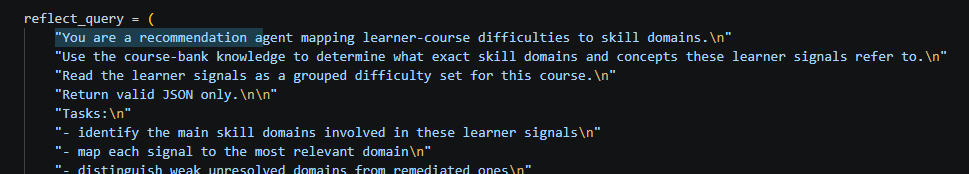
\includegraphics[width=0.75\textwidth]{figures/system_prompt_agent_defis.png}
}{%
    \fbox{\parbox{0.85\textwidth}{\centering Capture du prompt système de l'Agent de recommandation à insérer ici.}}
}
\caption{Exemple de prompt système utilisé par l'Agent de recommandation}
\label{fig:system_prompt_agent_recommandation}
\end{figure}

\subsection{Les agent skills}

Cette section présente les agent skills et leur intégration dans la plateforme.

\subsubsection{Définition}

Les agent skills \cite{agent_skills_overview} désignent des blocs d'instructions spécialisés
qu'un agent peut utiliser pour traiter une tâche précise. Contrairement au prompt système,
qui définit le comportement général de l'agent, un skill apporte une logique plus ciblée :
il précise une méthode de raisonnement, des règles de décision ou une procédure adaptée à
un cas particulier.

\subsubsection{Besoin des skills dans le projet}

Dans le cadre de ce projet, l'utilisation des skills permet d'éviter de centraliser l'ensemble des règles de fonctionnement dans un seul prompt système. Cette approche rend les agents plus modulaires et facilite leur évolution.

Lorsqu'une tâche spécifique doit être exécutée, l'agent peut activer uniquement le skill correspondant, sans alourdir son contexte avec des instructions inutiles. Cela permet une meilleure séparation des responsabilités et une organisation plus claire du comportement des agents.

Ainsi, les skills contribuent à structurer les logiques de traitement de manière indépendante, tout en améliorant la maintenabilité et la flexibilité du système.

% ------------------------------------------------------------
\section{Système de mémoire persistante des agents IA}

La mémoire persistante permet aux agents IA de conserver et réutiliser des informations au-delà d'une seule session. Dans la plateforme, elle sert à exploiter le parcours de l'apprenant, ses interactions et les contenus déjà traités.

Cette section présente la solution retenue pour la gestion de cette mémoire, son fonctionnement et son intégration dans l'architecture de la plateforme.

\subsection{Présentation de Hindsight}

Hindsight \cite{hindsight_github} est un système de mémoire conçu pour les agents IA. Il fournit une couche dédiée à la mémorisation, à la récupération et à l'exploitation des informations retenues au fil des interactions, permettant ainsi de construire une mémoire durable et réutilisable.

Dans ce projet, Hindsight est retenu comme solution de mémoire persistante pour les agents IA, afin de conserver un contexte exploitable au fil des interactions et de renforcer la continuité des traitements.

\subsection{Architecture générale de Hindsight}

L'architecture de Hindsight repose sur deux niveaux principaux. Le premier correspond à la couche d'intégration, permettant aux agents de communiquer avec le système via une API, un SDK ou un client. Cette couche expose les opérations essentielles de gestion de mémoire telles que \textit{retain}, \textit{recall} et \textit{reflect}. Le second niveau est la couche de mémoire, organisée en \textit{memory banks} afin d'isoler les contextes selon l'utilisateur, le domaine ou le cours.

Au sein de chaque \textit{memory bank}, les informations sont structurées sous forme d'unités enrichies contenant des entités, des relations et des données temporelles. Ces éléments sont ensuite consolidés en différentes formes de connaissances, allant de faits simples à des représentations contextuelles plus globales (Figure~2.3).

\begin{figure}[H]
\centering
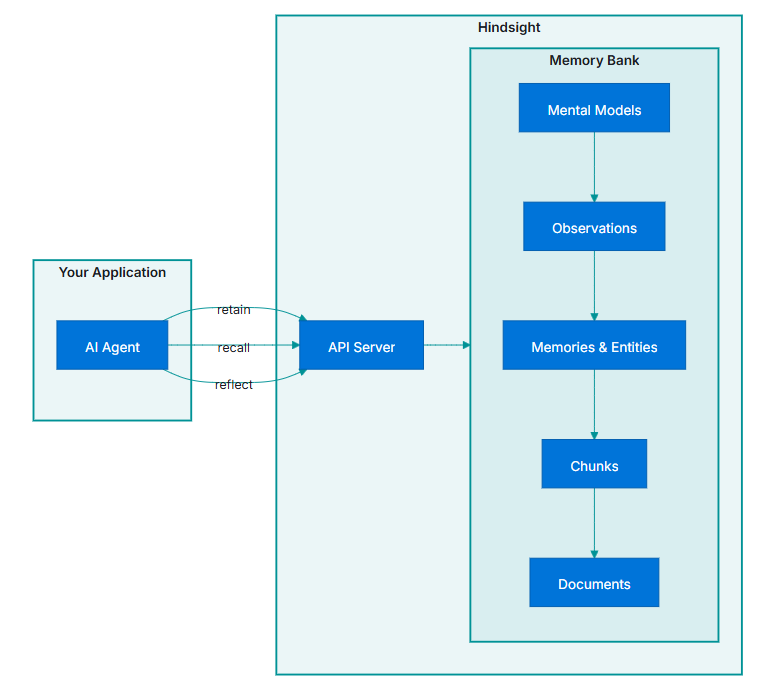
\includegraphics[width=0.75\textwidth]{figures/hindsight_architecture.png}
\caption{Architecture conceptuelle de Hindsight \cite{hindsight_homepage}}
\label{fig:hindsight_architecture}
\end{figure}

\subsection{Fonctionnalités fondamentales utilisées}

Dans le cadre du projet, Hindsight s'appuie sur trois opérations principales : \textit{retain}, \textit{recall} et \textit{reflect}, couvrant l'ensemble du cycle de gestion de la mémoire.

\textbf{Retain :} cette opération correspond à l'enregistrement des informations dans la mémoire. Comme illustré à la Figure~\ref{fig:hindsight_retain_architecture}, le système ne stocke pas le texte brut, mais exploite un LLM pour extraire les informations importantes (faits, entités, contexte temporel), puis les normalise afin d'éviter les doublons. Ces données sont transformées en \textit{memory units} enrichies par des métadonnées et des embeddings, puis organisées et classées en différentes catégories (\textit{world}, \textit{experience}, \textit{opinion}, \textit{observation}) avant stockage. Dans la plateforme, cette opération permet de conserver les interactions de l'apprenant, ses difficultés, ses erreurs récurrentes et ses préférences.

\begin{center}
    \IfFileExists{figures/hindsight_retain_architecture.png}{%
        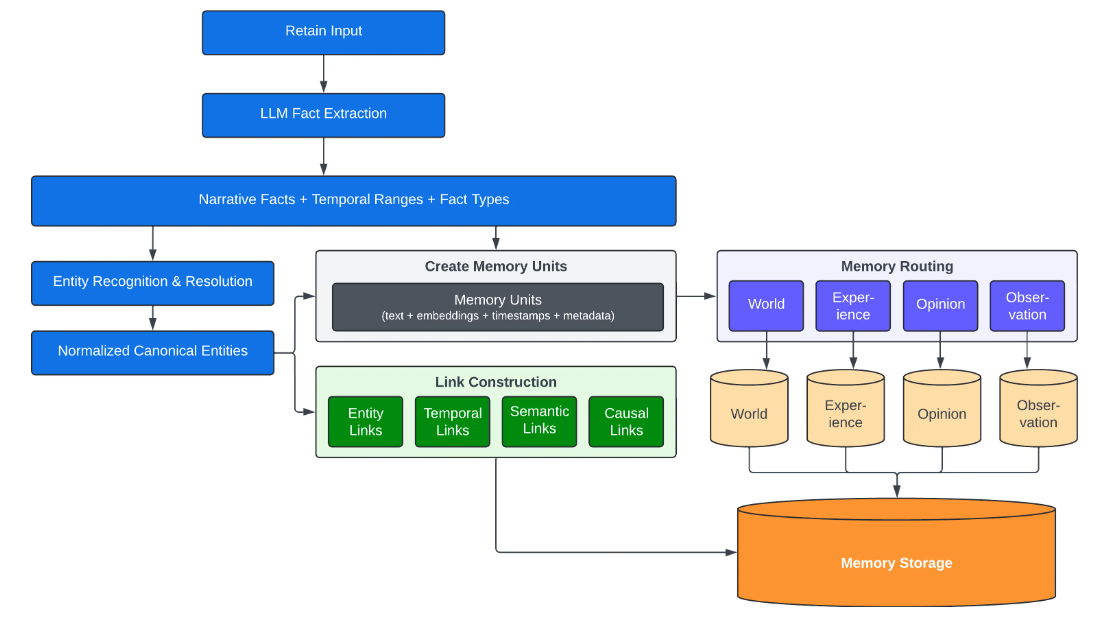
\includegraphics[width=0.98\textwidth]{figures/hindsight_retain_architecture.png}
    }{%
        \fbox{\parbox{0.85\textwidth}{\centering Schéma de fonctionnement de l'opération Retain à insérer ici.}}
    }
    \captionof{figure}{Fonctionnement de l'opération \textit{Retain} dans Hindsight \cite{hindsight_github}}
    \label{fig:hindsight_retain_architecture}
\end{center}

\textbf{Recall :} cette opération correspond à la récupération intelligente des mémoires déjà stockées. Comme l'illustre la figure \ref{fig:hindsight_recall_architecture}, Hindsight ne renvoie pas toute la mémoire à l'agent : il lance plusieurs recherches en parallèle, notamment la recherche sémantique par similarité vectorielle, la recherche par mots-clés, l'exploration des liens entre entités et l'exploitation des informations temporelles. Les résultats obtenus sont ensuite fusionnés, réordonnés et filtrés selon le budget de tokens disponible, afin de constituer un ensemble de souvenirs contextualisés à transmettre au LLM \cite{hindsight_recall}. Dans ce projet, \textit{recall} permet donc de retrouver les informations les plus utiles sur l'apprenant, son historique et le cours avant la génération d'une réponse.

\begin{center}
    \IfFileExists{figures/hindsight_recall_architecture.png}{%
        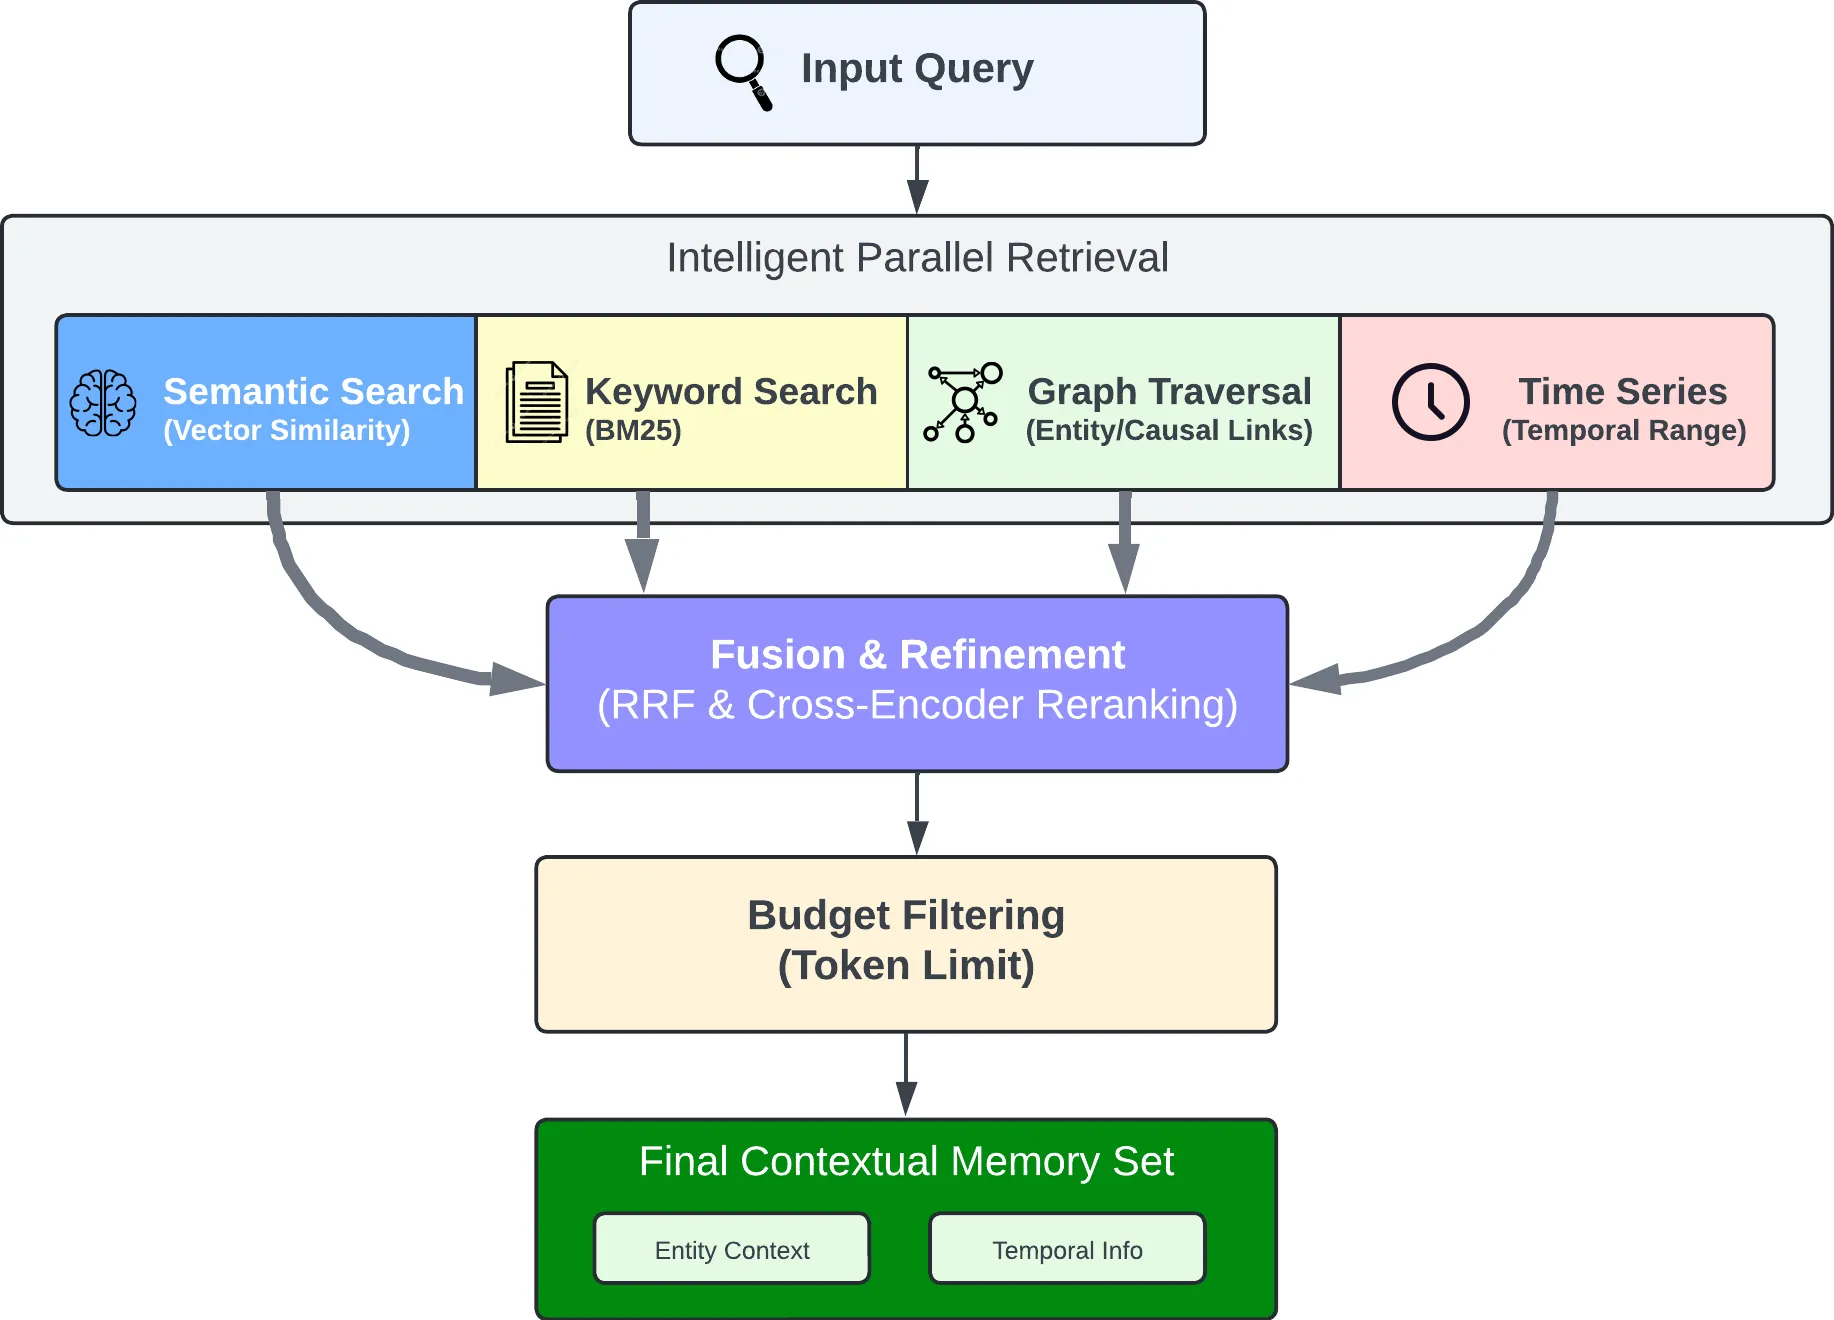
\includegraphics[width=0.9\textwidth]{figures/hindsight_recall_architecture.png}
    }{%
        \fbox{\parbox{0.85\textwidth}{\centering Schéma de fonctionnement de l'opération Recall à insérer ici.}}
    }
    \captionof{figure}{Fonctionnement de l'opération \textit{Recall} dans Hindsight \cite{hindsight_github}}
    \label{fig:hindsight_recall_architecture}
\end{center}

\noindent\textbf{Reflect :} cette opération correspond à la phase de réflexion et de mise à jour de la mémoire après une interaction. Comme l'illustre la figure \ref{fig:hindsight_reflect_architecture}, Hindsight récupère d'abord les mémoires pertinentes, construit un contexte, charge le profil de l'agent, puis utilise le LLM pour générer une réponse cohérente avec ce contexte. La réponse produite est ensuite analysée afin d'identifier de nouvelles observations ou de mettre à jour des opinions existantes, avec un niveau de confiance associé. Ces éléments sont réinjectés dans la mémoire persistante, ce qui permet à l'agent d'améliorer progressivement la cohérence de ses futures interactions \cite{hindsight_reflect}. Dans ce projet, \textit{reflect} est utile pour dégager des tendances sur le parcours d'un apprenant, consolider des observations pédagogiques et enrichir la mémoire des agents au fil des échanges.

\begin{center}
    \IfFileExists{figures/hindsight_reflect_architecture.png}{%
        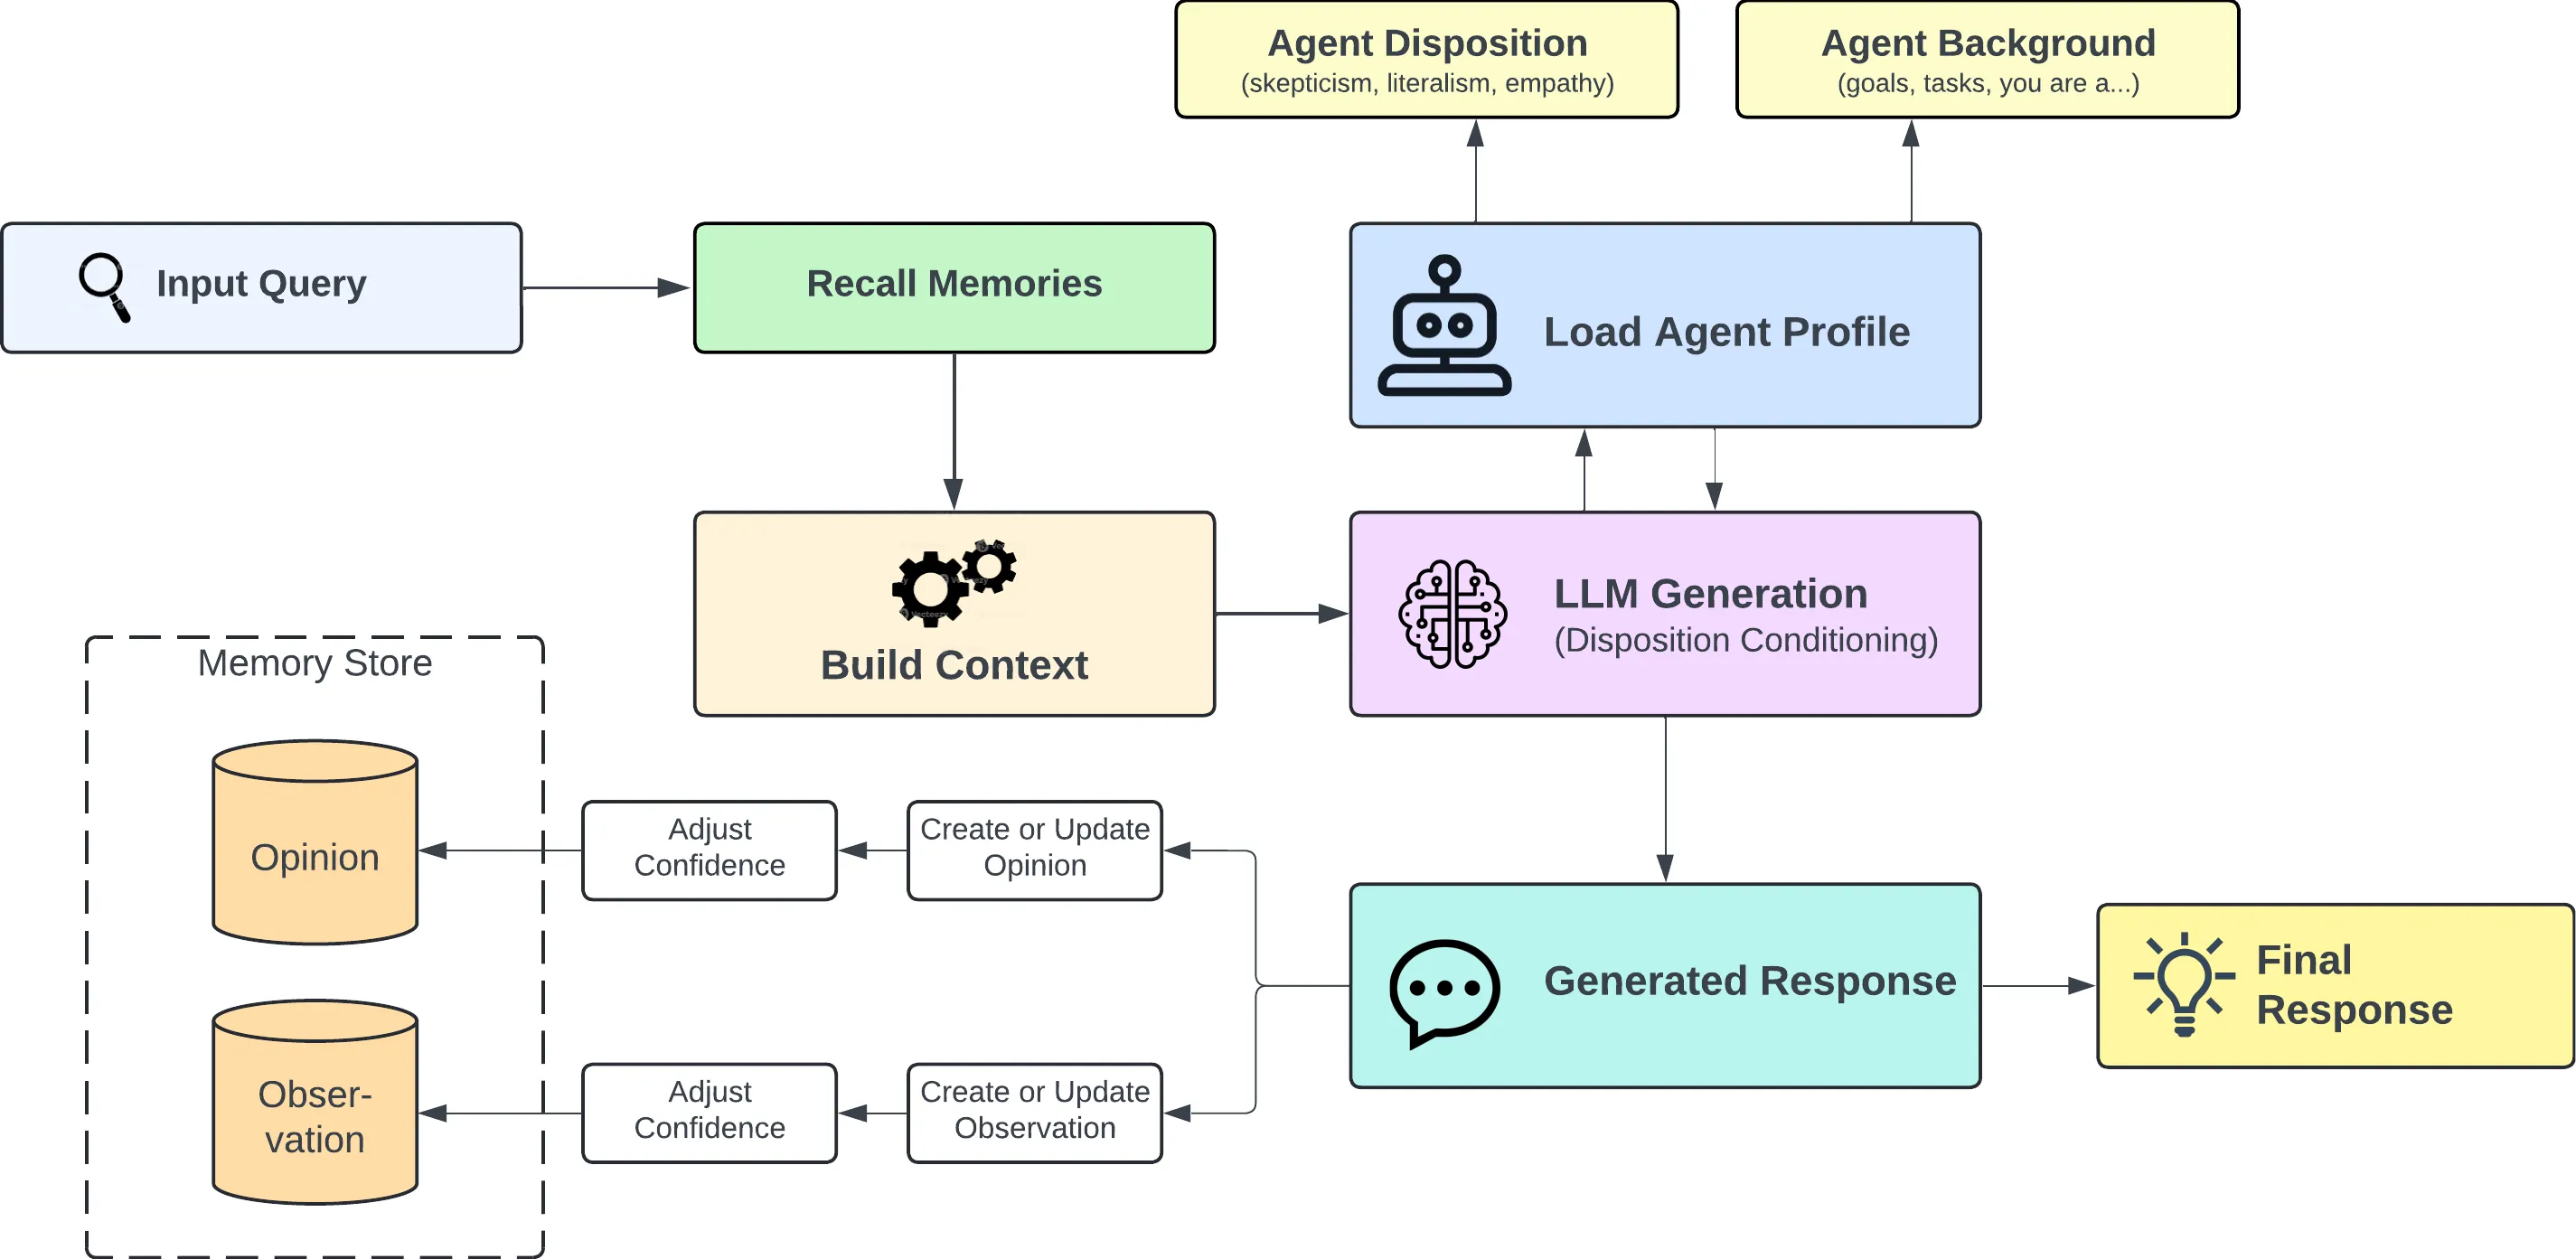
\includegraphics[width=0.9\textwidth]{figures/hindsight_reflect_architecture.png}
    }{%
        \fbox{\parbox{0.85\textwidth}{\centering Schéma de fonctionnement de l'opération Reflect à insérer ici.}}
    }
    \captionof{figure}{Fonctionnement de l'opération \textit{Reflect} dans Hindsight \cite{hindsight_github}}
    \label{fig:hindsight_reflect_architecture}
\end{center}

En résumé, l'organisation de la mémoire Hindsight repose sur un cycle continu qui permet
de conserver, d'exploiter et d'améliorer progressivement les informations utiles aux agents IA.
Cette approche donne à la plateforme une mémoire durable, capable de maintenir le contexte
au fil des interactions et de soutenir une personnalisation plus cohérente des réponses, des
recommandations et des activités proposées.



\subsection{Structure des mémoires persistantes dans Hindsight}

Dans ce projet, Hindsight organise les informations sous forme de \textit{memory banks} séparées, indexées à partir du \textit{tenantId}, du \textit{userId} et du \textit{courseId}. Cette organisation permet d'isoler les contextes (organisation, apprenant, cours) et d'offrir aux agents une mémoire structurée et ciblée. Le préfixe \texttt{tenant:\{tenantId\}} garantit également la cohérence avec l'architecture multi-tenant et évite tout mélange entre environnements.

On distingue principalement quatre types de banques mémoire :

\begin{itemize}
    \item \textbf{Banque de cours} \\
    \texttt{tenant:\{tenantId\}:course:\{courseId\}} \\
    Elle contient la mémoire pédagogique stable du cours (objectifs, leçons, quiz, supports, concepts). Elle est alimentée après la publication du cours et utilisée par les agents de coaching, recommandation et défis.

    \item \textbf{Banque apprenant-cours} \\
    \texttt{tenant:\{tenantId\}:user:\{userId\}:course:\{courseId\}} \\
    Elle regroupe l'historique de l'apprenant dans un cours (progression, résultats, erreurs, difficultés, interactions et retours).

    \item \textbf{Banque générale de l'apprenant} \\
    \texttt{tenant:\{tenantId\}:user:\{userId\}} \\
    Elle stocke les informations transversales comme les préférences pédagogiques, le profil et les connaissances générales.

    \item \textbf{Banque de profil de compétences} \\
    \texttt{tenant:\{tenantId\}:user:\{userId\}:skill-profile} \\
    Elle contient une synthèse des compétences et des écarts, utilisée principalement par l'Agent de recommandation pour éviter les recalculs.
\end{itemize}

Ainsi, cette structuration sépare clairement les connaissances liées au cours, au parcours utilisateur et aux compétences. Elle améliore la lisibilité de la mémoire, limite les ambiguïtés et permet aux agents de sélectionner directement le contexte pertinent selon leur objectif.


\section{Conclusion}

Ce chapitre a permis de poser les bases théoriques nécessaires à la compréhension de la solution proposée. Ces fondements constituent le socle sur lequel repose l'ensemble des mécanismes d'intelligence et d'interaction de la plateforme.

Ils offrent ainsi une vision claire des principes qui guident la conception et la mise en œuvre du système dans la suite du projet.

